\documentclass[a4paper,11pt]{exam}
\printanswers % pour imprimer les réponses (corrigé)
%\noprintanswers % Pour ne pas imprimer les réponses (énoncé)
\addpoints % Pour compter les points
% \noaddpoints % pour ne pas compter les points
%\qformat{\textbf{\thequestion ) } }
%\qformat{\textbf{\thequestion )}} % Pour définir le style des questions (facultatif)
\usepackage{color} % définit une nouvelle couleur
\shadedsolutions % définit le style des réponses
% \framedsolutions % définit le style des réponses
\definecolor{SolutionColor}{rgb}{0.8,0.9,1} % bleu ciel
\renewcommand{\solutiontitle}{\noindent\textbf{Solution:}\par\noindent} % Définit le titre des solutions
\usepackage{gensymb}



\makeatletter

\def\maketitle{{\centering%
	\par{\huge\textbf{\@title}}%
	\par{\@date}%
	\par}}


\renewcommand{\thesubsection}{\Alph{subsection}.}   

\makeatother

\lhead{NOM Pr\'enom :}
\rhead{\textbf{Les r\'eponses doivent \^etre justifi\'ees et r\'edig\'ees}}
\cfoot{\thepage / \pageref{LastPage}}


%\usepackage{../../pas-math}
%\usepackage{../../moncours}


%\usepackage{pas-cours}
%-------------------------------------------------------------------------------
%          -Packages nécessaires pour écrire en Français et en UTF8-
%-------------------------------------------------------------------------------
\usepackage[utf8]{inputenc}
\usepackage[frenchb]{babel}
%\usepackage{numprint}
\usepackage[T1]{fontenc}
%\usepackage{lmodern}
\usepackage{textcomp}
\usepackage[french, boxed]{algorithm2e}
\usepackage{hyperref}


%-------------------------------------------------------------------------------

%-------------------------------------------------------------------------------
%                          -Outils de mise en forme-
%-------------------------------------------------------------------------------
\usepackage{hyperref}
\hypersetup{pdfstartview=XYZ}
%\usepackage{enumerate}
\usepackage{graphicx}
\usepackage{multicol}
\usepackage{tabularx}
\usepackage{multirow}
\usepackage{color}
\usepackage{eurosym}


\usepackage{anysize} %%pour pouvoir mettre les marges qu'on veut
%\marginsize{2.5cm}{2.5cm}{2.5cm}{2.5cm}

\usepackage{indentfirst} %%pour que les premier paragraphes soient aussi indentés
\usepackage{verbatim}
\usepackage{enumitem}
\usepackage{booktabs}
\usepackage[usenames,dvipsnames,svgnames,table]{xcolor}

\usepackage{variations}

%-------------------------------------------------------------------------------


%-------------------------------------------------------------------------------
%                  -Nécessaires pour écrire des mathématiques-
%-------------------------------------------------------------------------------
\usepackage{amsfonts}
\usepackage{amssymb}
\usepackage{amsmath}
\usepackage{amsthm}
\usepackage{tikz}
\usepackage{xlop}
\usepackage[output-decimal-marker={,}]{siunitx}
%-------------------------------------------------------------------------------

%-------------------------------------------------------------------------------
%                  -Nécessaires pour écrire des formules chimiquess-
%-------------------------------------------------------------------------------

\usepackage[version=4]{mhchem}

%-------------------------------------------------------------------------------
% Pour pouvoir exploiter les fichiers directement dans beamer
\newcommand{\pause}{\ }
%-------------------------------------------------------------------------------
%                    - Mise en forme avancée
%-------------------------------------------------------------------------------

\usepackage{ifthen}
\usepackage{ifmtarg}


\newcommand{\ifTrue}[2]{\ifthenelse{\equal{#1}{true}}{#2}{$\qquad \qquad$}}

%\newcommand{\kword}[1]{\textcolor{red}{\underline{#1}}}
%-------------------------------------------------------------------------------

%-------------------------------------------------------------------------------
%                     -Mise en forme d'exercices-
%-------------------------------------------------------------------------------
%\newtheoremstyle{exostyle}
%{\topsep}% espace avant
%{\topsep}% espace apres
%{}% Police utilisee par le style de thm
%{}% Indentation (vide = aucune, \parindent = indentation paragraphe)
%{\bfseries}% Police du titre de thm
%{.}% Signe de ponctuation apres le titre du thm
%{ }% Espace apres le titre du thm (\newline = linebreak)
%{\thmname{#1}\thmnumber{ #2}\thmnote{. \normalfont{\textit{#3}}}}% composants du titre du thm : \thmname = nom du thm, \thmnumber = numéro du thm, \thmnote = sous-titre du thm

%\theoremstyle{exostyle}
%\newtheorem{exercice}{Exercice}
%
%\newenvironment{questions}{
%\begin{enumerate}[\hspace{12pt}\bfseries\itshape a.]}{\end{enumerate}
%} %mettre un 1 à la place du a si on veut des numéros au lieu de lettres pour les questions 
%-------------------------------------------------------------------------------

%-------------------------------------------------------------------------------
%                    - Mise en forme de tableaux -
%-------------------------------------------------------------------------------

\renewcommand{\arraystretch}{1.7}

\setlength{\tabcolsep}{1.2cm}

%-------------------------------------------------------------------------------



%-------------------------------------------------------------------------------
%                    - Racourcis d'écriture -
%-------------------------------------------------------------------------------
%Droites
\newcommand{\dte}[1]{$(#1)$}
\newcommand{\fig}[1]{figure $#1$}
\newcommand{\sym}{symétrique}
\newcommand{\syms}{symétriques}
\newcommand{\asym}{axe de symétrie}
\newcommand{\asyms}{axes de symétrie}
\newcommand{\seg}[1]{$[#1]$}
\newcommand{\monAngle}[1]{$\widehat{#1}$}
\newcommand{\bissec}{bissectrice}
\newcommand{\mediat}{médiatrice}
\newcommand{\ddte}[1]{$[#1)$}


% Angles orientés (couples de vecteurs)
\newcommand{\aopp}[2]{(\vec{#1}, \vec{#2})} %Les deuc vecteurs sont positifs
\newcommand{\aopn}[2]{(\vec{#1}, -\vec{#2})} %Le second vecteur est négatif
\newcommand{\aonp}[2]{(-\vec{#1}, \vec{#2})} %Le premier vecteur est négatif
\newcommand{\aonn}[2]{(-\vec{#1}, -\vec{#2})} %Les deux vecteurs sont négatifs

%Ensembles mathématiques
\newcommand{\naturels}{\mathbb{N}} %Nombres naturels
\newcommand{\relatifs}{\mathbb{Z}} %Nombres relatifs
\newcommand{\rationnels}{\mathbb{Q}} %Nombres rationnels
\newcommand{\reels}{\mathbb{R}} %Nombres réels
\newcommand{\complexes}{\mathbb{C}} %Nombres complexes


%Intégration des parenthèses aux cosinus
\newcommand{\cosP}[1]{\cos\left(#1\right)}
\newcommand{\sinP}[1]{\sin\left(#1\right)}


%Probas stats
\newcommand{\stat}{statistique}
\newcommand{\stats}{statistiques}


\newcommand{\homo}{homothétie}
\newcommand{\homos}{homothéties}


\newcommand{\mycoord}[3]{(\textcolor{red}{\num{#1}} ; \textcolor{Green}{\num{#2}} ; \textcolor{blue}{\num{#3}})}
%-------------------------------------------------------------------------------

%-------------------------------------------------------------------------------
%                    - Mise en page -
%-------------------------------------------------------------------------------

\newcommand{\twoCol}[1]{\begin{multicols}{2}#1\end{multicols}}


\setenumerate[1]{font=\bfseries,label=\textit{\alph*})}
\setenumerate[2]{font=\bfseries,label=\arabic*)}


%-------------------------------------------------------------------------------
%                    - Elements cours -
%-------------------------------------------------------------------------------

%Correction d'exercice
\newcommand{\exoSec}[2]{\subsection*{Exercice #1 page #2}}
%-------------------------------------------------------------------------------
%                    - raccourcis d'écriture -
%-------------------------------------------------------------------------------

%Mise en évidence de termes clés
\newcommand{\mykw}[1]{\textcolor{red}{\underline{\textbf{#1}}}}

%Exercices
\newcommand{\exo}[2]{exercice #1 page #2}
\newcommand{\Exo}[2]{Exercice #1 page #2}

\renewcommand{\pause}{\ }

%Intervalles
\newcommand{\interOO}[2]{$]$#1 , #2$[$}
\newcommand{\interOF}[2]{$]$#1 , #2$]$}
\newcommand{\interFO}[2]{$[$#1 , #2$[$}
\newcommand{\interFF}[2]{$[$#1 , #2$]$}



%\usepackage{fullpage}
\author{\ }
\date{24 Septembre 2018}
\title{Sciences Physiques : DS n° 1}


\begin{document}
%	\usepackage{fancyhdr}
%	
%	\pagestyle{fancy}
%	\fancyhf{}
	%\rhead{Share\LaTeX}

	\maketitle
	
\begin{small}
	\begin{center}
		\begin{tabular}{|@{\ }l@{}|@{\ }c@{\ }|}
			\hline
			\textbf{Compétence} & \textbf{Maitrise} \\
			\hline
			Exploiter des mesures de masse volumique pour différencier des espèces chimiques.\ &  \ \ \ \\
			\hline	
		\end{tabular}
	\end{center}
\end{small}	
	
	
%\vspace*{-0.5cm}	

%\section{\'Equations de réaction}

Ajuster les équations de réactions suivantes :
\begin{questions}
	\question $CH_4 + ....O_2 \rightarrow ....CO_2 + ....H_2O$
	
	\question $C_7H_{16} + ....O_2 \rightarrow ....CO_2 + ....H_2O$	
	
	\question $C_6H_{2}O + ....O_2 \rightarrow ....CO_2 + ....H_2O$
\end{questions}


%\section{À chaque modèle sa formule}
\begin{questions}
	\question \'A partir de ces dessins de modèles, donner la formule des molécules suivantes.

	\begin{center}
		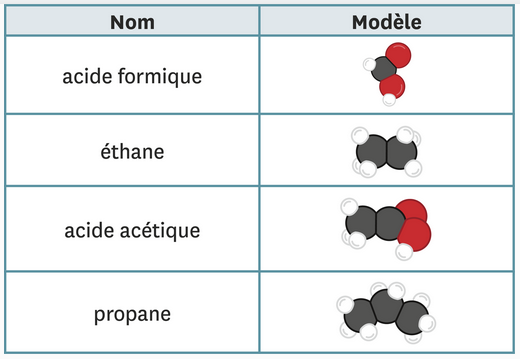
\includegraphics[scale=0.6]{img/exemples}
	\end{center}
	\fillwithdottedlines{2cm}
	
\end{questions}

Seul l'\ref{ex:qcm} est à faire sur le sujet. Le soin et la qualité de rédaction sont pris en compte dans la notation.


\section{QCM (3 points)}

Pour chaque question, choisir la (ou les) bonnes réponses

\begin{questions}
	
	\begin{multicols}{2}
		
		\question[\half] Le ballon de handball est en mouvement par rapport :
	
	
	
		
	\begin{checkboxes}
		\correctchoice au sol.
		\correctchoice à un joueur.
		\choice au ballon.
	\end{checkboxes}

	\begin{center}
		
\includegraphics[scale=0.3]{hand}
	\end{center}
	\end{multicols}

	\question[\half] La tour Eiffel est fixe par rapport :\\
	\begin{oneparcheckboxes}
		\choice à la Lune.
		\correctchoice à la surface de la Terre.
		\choice au Soleil
	\end{oneparcheckboxes}

	\question[\half] Les passagers d'une grande roue pendant son fonctionnement sont immobiles par rapport :
	\begin{oneparcheckboxes}
		\correctchoice à leur nacelle.
		\choice au sol.
		\choice au centre de la roue.
	\end{oneparcheckboxes}



	\begin{multicols}{2}
		\question[\half] L'image ci-dessous est une chronophotographie d'un saut en bmx. La trajectoire du casque par rapport au sol est :
	\begin{checkboxes}
		\correctchoice curviligne.
		\choice rectiligne.
		\choice circulaire.
	\end{checkboxes}

	
	\begin{center}
		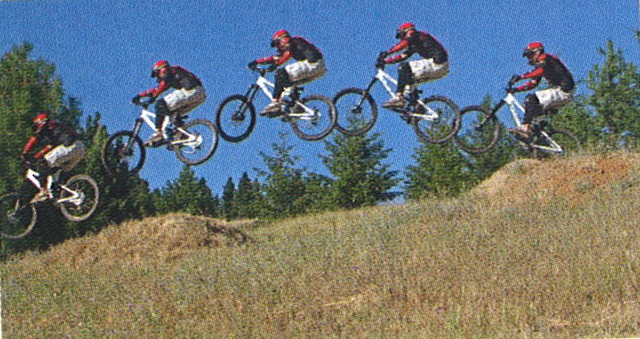
\includegraphics[scale=0.3]{bmx}
	\end{center}

	\end{multicols}
	\question[\half] La trajectoire de la nacelle d'une grande roue par rapport au sol est :\\
	\begin{oneparcheckboxes}
		\choice curviligne.
		\choice rectiligne.
		\correctchoice circulaire.
	\end{oneparcheckboxes}
	
	
	\begin{multicols}{2}
		\question[\half] La trajectoire du casque par rapport au centre de la Terre de ces enfants assis sur un banc est :
	\begin{checkboxes}
		\choice curviligne.
		\choice rectiligne.
		\correctchoice circulaire.
	\end{checkboxes}

	\begin{center}
		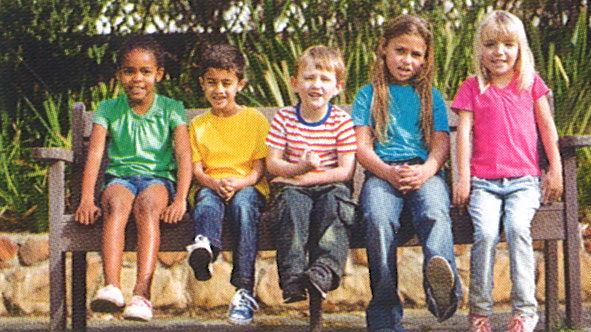
\includegraphics[scale=0.3]{banc}
	\end{center}
	\end{multicols}
\end{questions}

%\newpage





\section{Une bague en argent (4 points)}\label{ex:bague}

Florent observe la bague de Suzanne. Suzanne lui affirme que c'est une bague en argent mais Florent pense qu'elle est en fer-blanc. Pour en avoir le c\oe ur net, il pèse la bague et trouve $m = \num{14.4} \ g$. Il plonge la bague dans une éprouvette contenant$ \num{5.0} \ mL$ d'eau : le niveau monte jusqu'à $\num{6.4} \ mL$.  

\begin{questions}
	\question[1] De combien le volume d'eau dans l'éprouvette a-t-il augmenté ? En déduire la volume de la bague de Suzanne.
	\begin{solution}
		Le volume d'eau a augmenté de $\num{1.4} mL$, donc la bague a un volume de $\num{1.4} mL$, soit $\num{1.4} cm^3.$
	\end{solution}
	
	\question[1] A l'aide des données du tableau, calculer la masse que ferait la bague si elle était en fer-blanc.
	\begin{solution}
		\begin{equation*}
		\num{1.4} \times \num{8} = \num{11,2} 
		\end{equation*}
		
		Si elle était en argent la bague aurait une masse de $\num{11,2} g$. 
	\end{solution}
	
	\question[1] A l'aide du tableau, calculer la masse que ferait la bague si elle était en argent.
	\begin{solution}
		\begin{equation*}
		\num{1.4} \times \num{10.3} = \num{14,42} 
		\end{equation*}
		
		Si elle était en argent la bague aurait une masse de $\num{14,42} g$. 
	\end{solution}
	
	\question[1] Déterminer à l'aide des réponses précédentes, si la bague de Suzanne est en argent ou en fer-blanc.
	\begin{solution}
		La masse mesurée sur la balance est $\num{14,4} g$ donc la bague est argent, Suzanne a raison.
	\end{solution}

\end{questions}

\begin{center}
	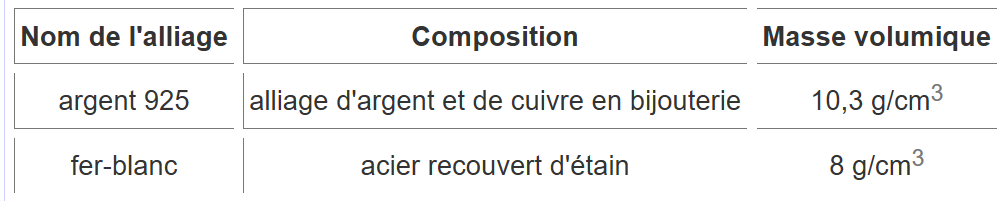
\includegraphics[scale=0.5]{img/tableau}
\end{center}




%\newpage

\section{Classement (2 points)}\label{ex:classement}

Soit huit échantillons de 10g de matériaux différents.

{\small \begin{center}
	\begin{tabular}{|@{\ }c@{\ }|@{\ }c@{\ }|}
		\hline
		\textbf{Matériau}  & \textbf{Masse volumique ($kg/m^3$)} \\ \hline
		diamant   & \num{3517}                 \\ \hline
		coton     & \num{40}                   \\ \hline
		acier     & \num{7800}                 \\ \hline
		bronze    & \num{8400}                 \\ \hline
		fer       & \num{7680}                 \\ \hline
		or        & \num{19300}                \\ \hline
		uranium   & \num{18700}                \\ \hline
		aluminium & \num{2700}                 \\ \hline
	\end{tabular}
\end{center}}

\begin{questions}
	\question[2] Classer les échantillons par ordre de volume croissant.
	
	\begin{solution}
		{\small \begin{center}
				\begin{tabular}{|@{\ }c@{\ }|@{\ }c@{\ }|@{\ }c@{\ }|@{\ }c@{\ }|@{\ }c@{\ }|}
					\hline
					\textbf{Matériau}  & \textbf{$\rho$ ($kg/m^3$)} & \textbf{$\rho$ ($g/m^3$)} & \textbf{$\rho$ ($g/cm^3$)} & Volume ($\frac{10}{\rho}$ ($cm^3$))   \\ \hline
					diamant   & \num{3517}  & \num{3517000} &  \num{3.517} & \num{2.84} \\ \hline
					coton     & \num{40}    & \num{40000}  & \num{0.04} & \num{250} \\ \hline
					acier     & \num{7800}  & \num{7800000}   & \num{7.8} & \num{1.28} \\ \hline
					bronze    & \num{8400}  & \num{8400000}   & \num{8.4} & \num{1.19} \\ \hline
					fer       & \num{7680}  & \num{7680000}  & \num{7.68} & \num{1.30} \\ \hline
					or        & \num{19300} & \num{19300000}  & \num{19.3} & \num{0.52} \\ \hline
					uranium   & \num{18700} & \num{18700000}  & \num{18.7} & \num{0.53} \\ \hline
					aluminium & \num{2700} & \num{2700000}    & \num{2.7} & \num{3.7} \\ \hline
				\end{tabular}
		\end{center}}
	
	D'où l'ordre suivant : or, uranium, bronze, acier, fer, diamant, aluminium, coton.
	\end{solution}
	
\end{questions}

%\newpage

\section{Conversions d'énergie}\label{ex:conversion}

\begin{questions}
	\question Quelle conversion d'énergie est réalisée par une éolienne ? par un ventilateur électrique ?
		\begin{solution}
			Une éolienne convertit l'énergie cinétique en énergie électrique. Un ventilateur convertit l'énergie électrique en énergie cinétique.
		\end{solution}
	
	\question Réaliser la chaine énergétique correspondant à l'éolienne.
		\begin{solution}
			\begin{center}
				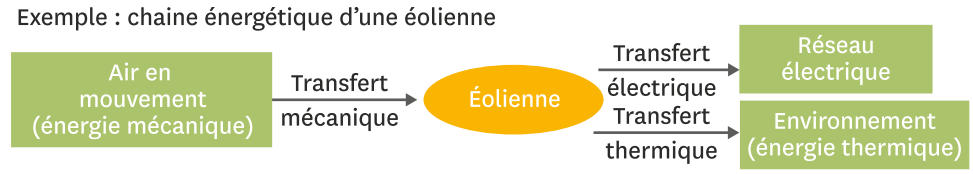
\includegraphics[scale=0.2]{img/chaine}
			\end{center}
		\end{solution}
	
\end{questions}

%\newpage 

%
\section{Monnaie en cuivre }

Au cours d'une opération de nettoyage de la plage, Romain a trouvé dix pièces de monnaie en cuivre. Il les plonge dans une éprouvette à moitié remplie d'eau. La différence de volume qu'il constate est $V = 5 cm^3$, il a trouvé sur internet que la masse volumique du cuivre est $\rho _{cuivre}$ est de $\num{8.96} g/mL$.  

\begin{questions}
	\question[] Convertir le volume $V$ des pièces de cuivre en mL.
	
	\question[] Calculer la masse $m$ de ces dix pièces de cuivre.
	
\end{questions}


%\newpage 

\section{Ordre de grandeur (5 points)}\label{ex:grandeur}

Le fer a longtemps été utilisé dans la fabrication d'objets quotidiens et a servi à la réalisation de grands projets urbains de l'aire industrielle. Sachant que la masse volumique du fer est de l'ordre de 8 $g/cm^3$, donner une estimation du volume de fer nécessaire à la fabrication des objets suivants :

\begin{enumerate}
	\item[1] Un clou d'une masse approximative de 12 g.
	
	\begin{solution}
		\begin{equation}
			12 \div 8 = 1.5
		\end{equation}
		
		Il faut \num{1.5} $cm^3$ de fer pour fabriquer un clou.
	\end{solution}
	
	\item[1] Un fer à cheval d'une masse approximative de 500 g.
	\begin{solution}
		\begin{equation}
			500 \div 8 = \num{62.5}
		\end{equation}
		
		Il faut \num{62.5} $cm^3$ de fer pour fabriquer un fer à cheval.
	\end{solution}

	\item[1] Un fer à repasser d'une masse approximative de 1 kg.
	\begin{solution}
		\begin{equation}
			1000 \div 8 = \num{125}
		\end{equation}
		
		Il faut \num{125} $cm^3$ de fer pour fabriquer un fer à repasser.
	\end{solution}

	\item[1] Un portail en fer forgé d'une masse approximative de 250 kg.
	\begin{solution}
		\begin{equation}
			125 \times 250 = \num{31250}
		\end{equation}
		
		Il faut \num{31250} $cm^3$ de fer pour fabriquer un portail, soit \num{31,250} $dm^3$.
	\end{solution}

	\item[1] La charpente métallique du pont Dom-Luis à Porto, dont la masse approximative est \num{3045} tonnes.
	\begin{solution}
		\begin{equation}
			\num{31250} \times 4 \times \num{3045} = \num{380625000}
		\end{equation}
		
		Il faut \num{380625000} $dm^3$ de fer pour fabriquer ce pont, soit \num{380625} $m^3$.
	\end{solution}
	
	
	
\end{enumerate}



 
%\newpage
%
%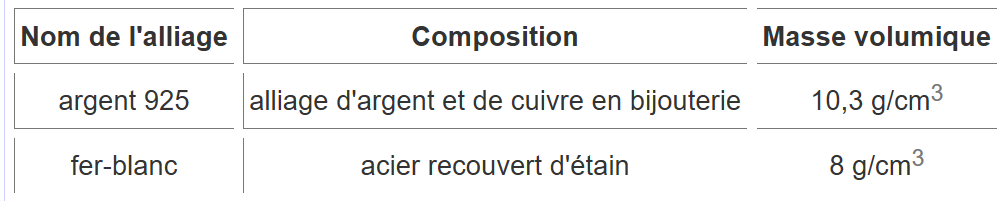
\includegraphics [scale=0.5, angle= 90 ]{img/tableau} 
\ \label{LastPage}

\end{document}